\newif\ifbaskerville \baskervilletrue

\documentclass[a4paper,11pt]{article}
\ifbaskerville
\usepackage{gill-sans,newbaskerville}
\renewcommand{\sfdefault}{gill-sans}
\fi
\usepackage{xcolor}
\usepackage{graphicx}
\usepackage[utf8]{inputenc}
\usepackage{enumitem} \setdescription{noitemsep}
\DeclareUnicodeCharacter{00A0}{~}
\setlength{\topmargin}{-2.5cm}
\setlength{\textheight}{26.5cm}
\setlength{\oddsidemargin}{-5mm}
\setlength{\textwidth}{17cm}
\pagestyle{empty}

\newcommand{\header}[4]{{\noindent \makebox[2cm][l]{ } \hfill 
    \hfill \makebox[2cm][r]{ } \vspace{-1ex} \\ \rule{\textwidth}{0pt}
    \begin{center} \Large\sffamily\bfseries #4 \end{center}} \vspace{5ex}}

\begin{document}
\header{Floorplan}{}{}{Hotel Cascais Miragem}
\label{Floorplan}

\paragraph{Gallery}
\begin{center}
  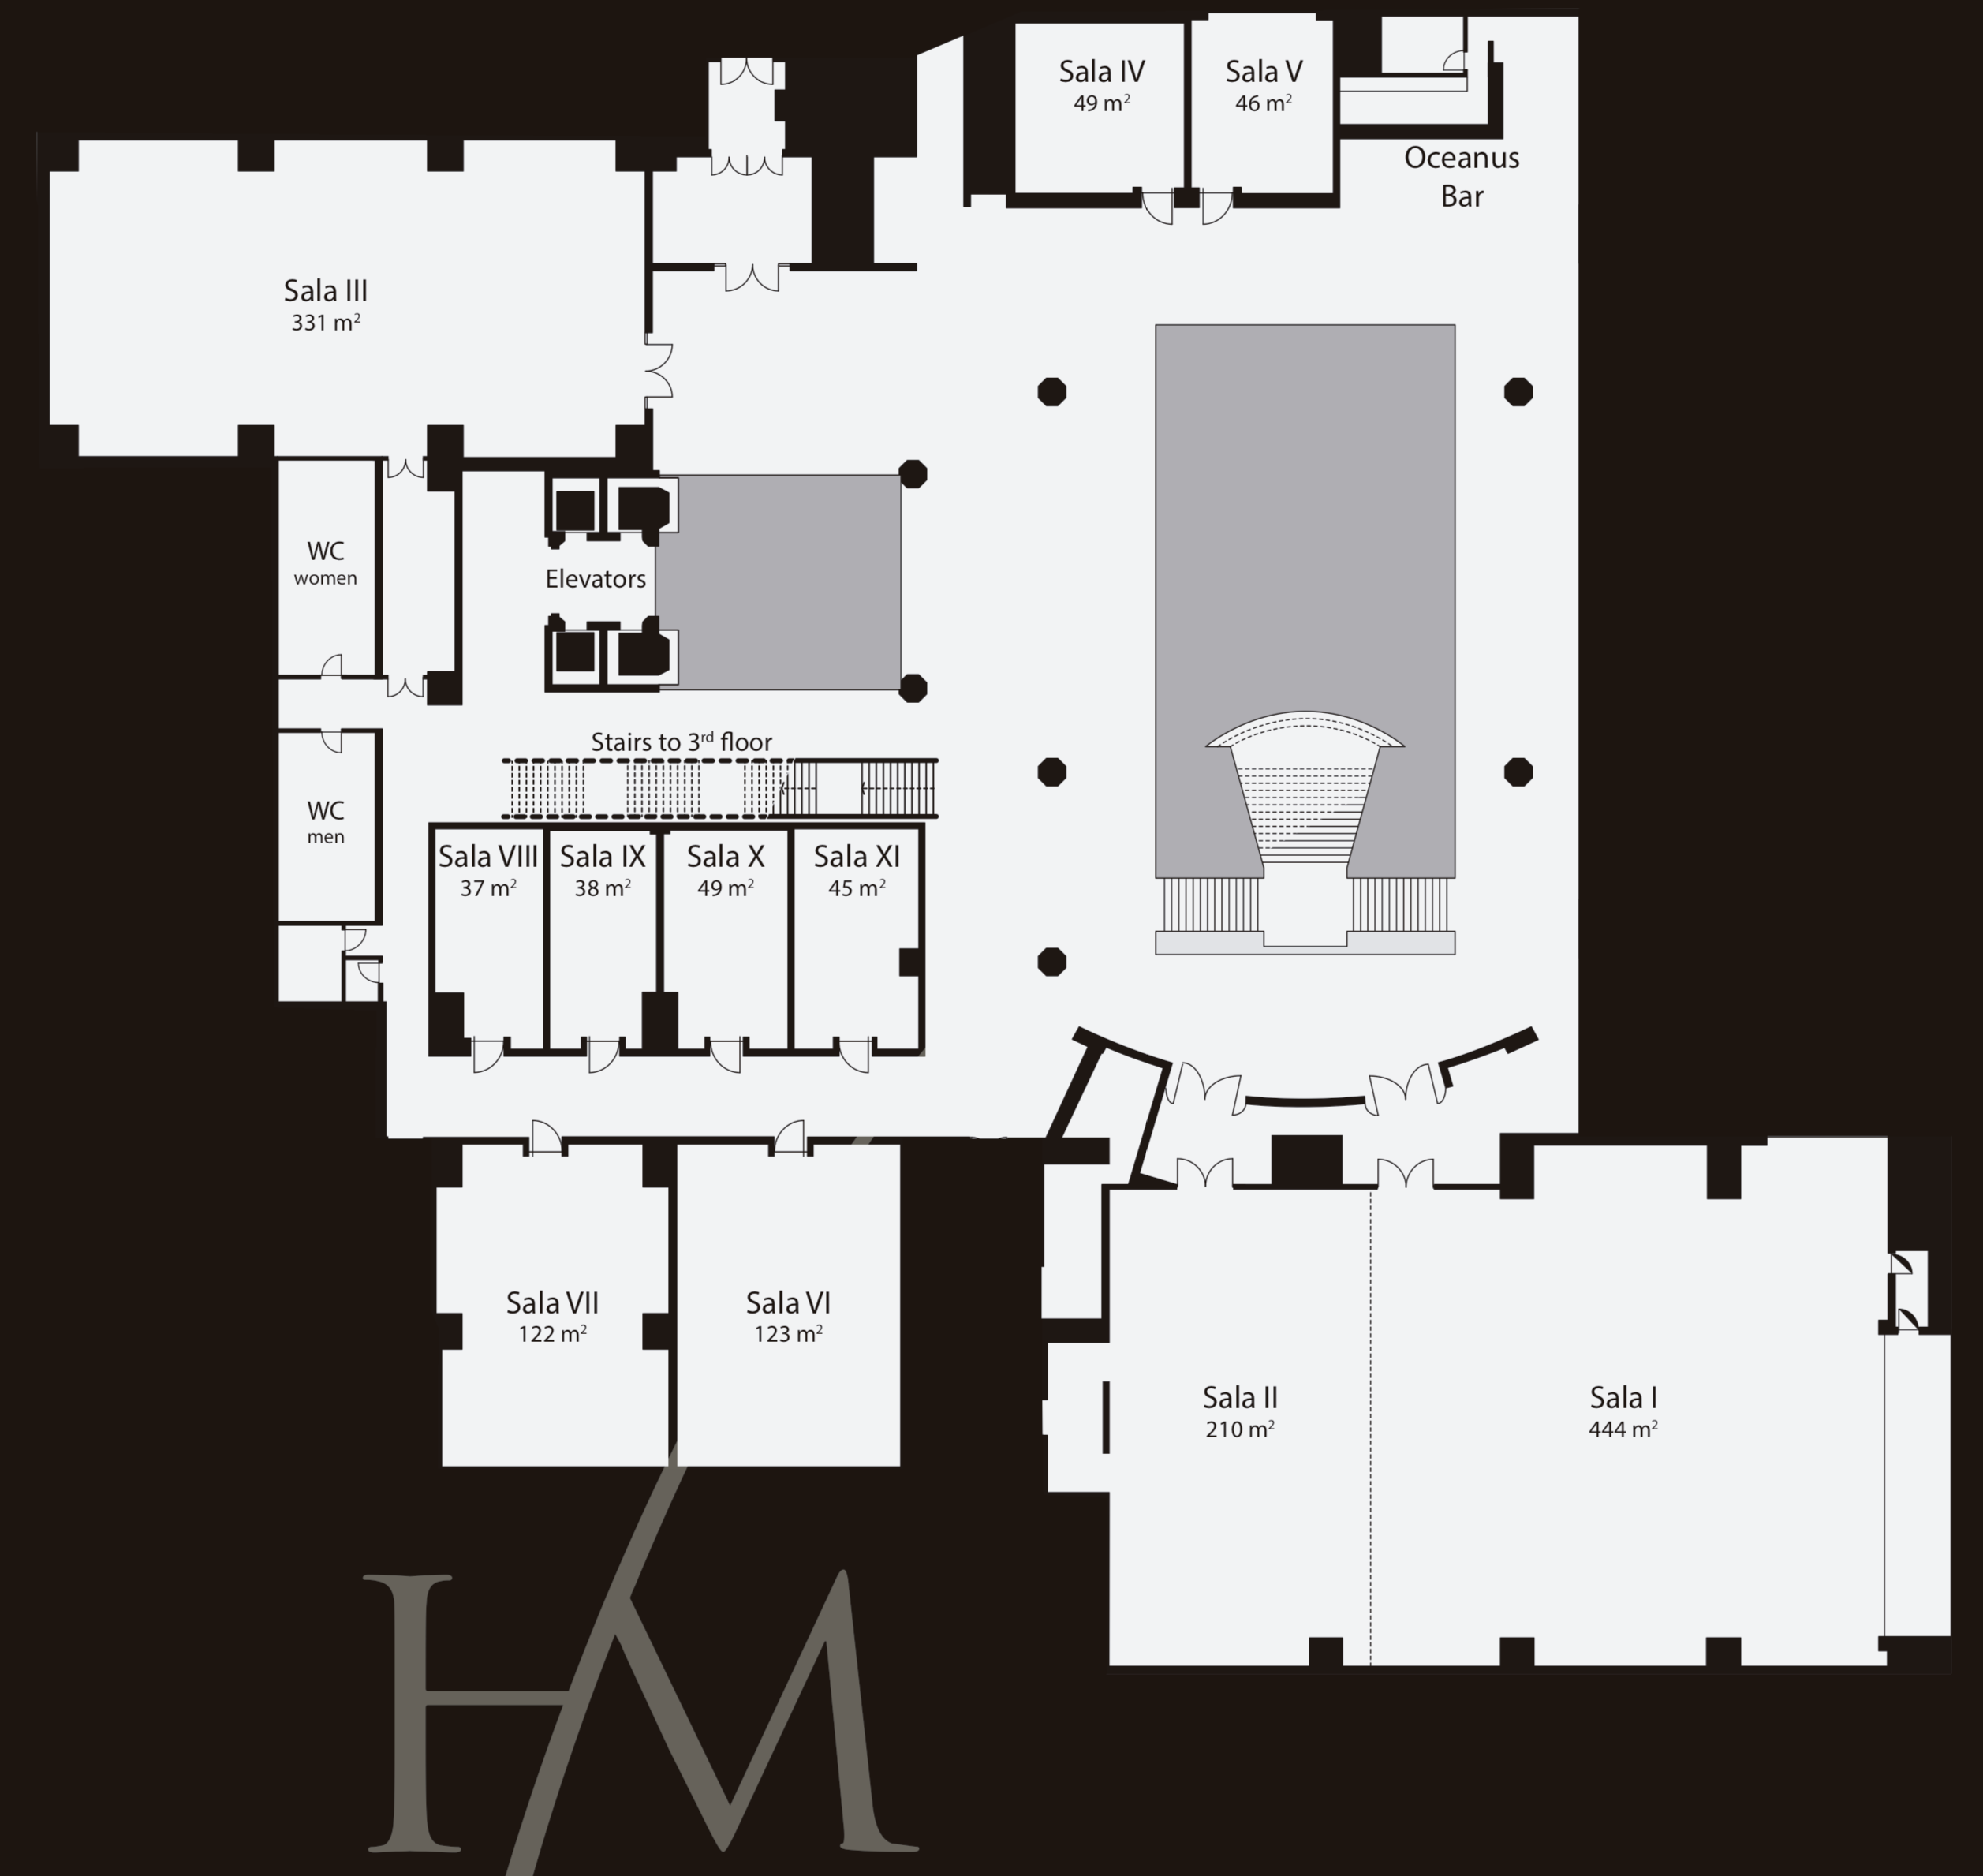
\includegraphics[width=0.7\textwidth]{img/gallery}
\end{center}

\paragraph{Lobby}
\begin{center}
  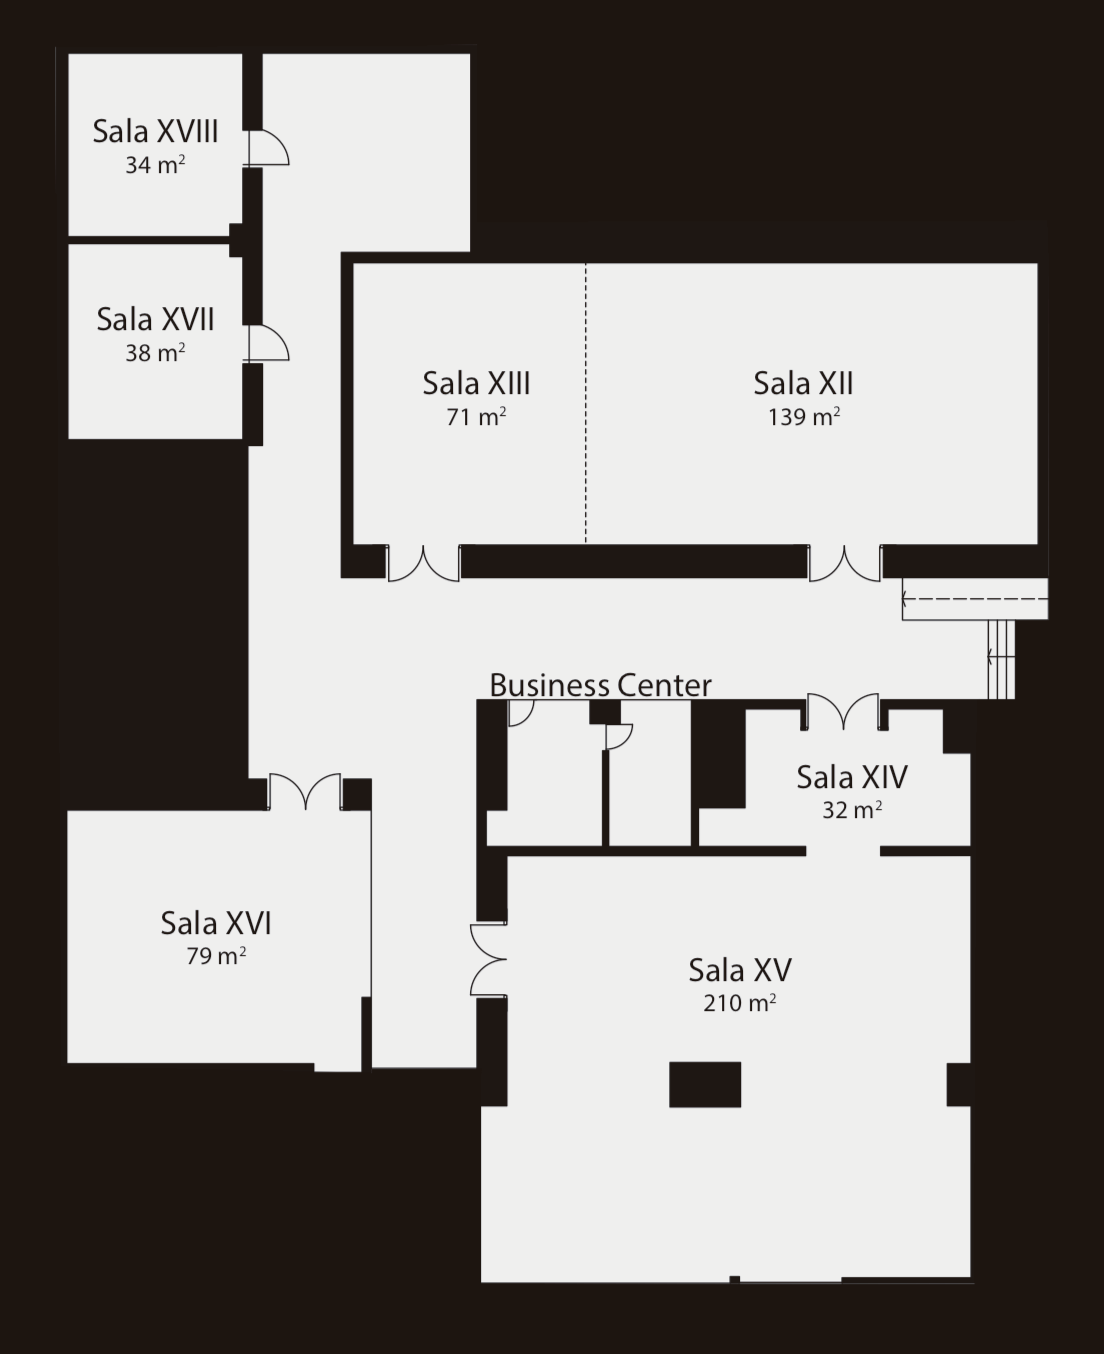
\includegraphics[width=0.35\textwidth]{img/lobby}
\end{center}

\vfil
\paragraph{WiFi}
\begin{description}
\item[SSID] \texttt{events}
\item[Password] \texttt{events2018}
\end{description}
% \begin{center}
% %\fbox{\Large\textbf{Wifi:} Connect to \textit{eduroam}, or sign up (for free) to \textit{The Cloud}.}
% \fbox{\Large\textbf{Wifi:} }
% \end{center}
\vfil
\eject

\newpage

%%% Local Variables:
%%% mode: latex
%%% TeX-master: t
%%% End:


\header{}{}{}{Location Map for Social Events}
\vfil
\includegraphics[width=\textwidth]{social-map.png}
\vfil
\end{document}
